\documentclass[aspectratio=169,11pt]{beamer}
\usepackage{teaching_slides}
\usepackage{listings}

\lstset{
  language=R,
  basicstyle=\ttfamily\tiny,
  backgroundcolor=\color{gray!5},
  frame=single,
  rulecolor=\color{gray!50},
  keywordstyle=\color{blue!70!black},
  commentstyle=\color{green!40!black},
  stringstyle=\color{orange!90!black},
  columns=flexible,
  keepspaces=true,
  showstringspaces=false,
  breaklines=true
}
\usepackage{inconsolata}

\title[L9b - Staggered DiD]{ Econometrics I}
\subtitle{Lecture 9b: Staggered Adoption and Modern Difference-in-Differences}
\author{Chris Conlon \\NYU Stern}
\date{Fall 2026}

% Rebuilt November 2026 (Session 9, second half; follows L9c). Simulation-first: a
% platform rolls an algorithm out city by city in four waves; the design deliberately
% differs from Assignment 5's. Goodman-Bacon, Callaway-Sant'Anna and imputation are
% coded by hand in staggered_sims.R and checked against two-way FE and sunab().
% Readings: Mixtape (Remix) Ch. 8b; Roth, Sant'Anna, Bilinski and Poe (2023, JoE).
% Figures/tables: staggered_sims.R. Workbook: Fall/L9 - Quasi Experiments/inclass_session9.Rmd, Part 2.

\begin{document}
\maketitle


\begin{frame}{Where we are}
\begin{itemize}
	\item Lecture 9a: one treatment date, a $2\times2$ comparison, parallel trends. Two-way FE got it exactly right.
	\medskip
	\item Most real rollouts are \alert{staggered}: firms, stores or markets adopt at different dates.
	\medskip
	\item The default is to run the same two-way FE regression with $D_{it}$ switching on at each unit's date.
	\begin{itemize}
		\item What does that coefficient estimate when effects differ across cohorts or grow over time?
		\item Which estimators fix it, and what do they assume?
		\item Does it matter in published work?
	\end{itemize}
	\medskip
	\item Plan: diagnose with a simulation where we know the answer, take the regression apart (FWL, then
	Goodman-Bacon), then rebuild it from clean $2\times2$s.
\end{itemize}
\end{frame}


\begin{frame}{Running example: an algorithm rolled out city by city}
\begin{itemize}
	\item A delivery platform launches a new recommendation algorithm in 300 cities over 20 months: four waves of
	60 cities (months 6, 9, 12 and 15), plus 60 cities that never get it. Outcome: log orders per user.
	\item Truth: nothing happens before launch. The effect ramps in over eight months, and earlier waves gain more
	(long-run effects 0.12, 0.09, 0.06, 0.04). The platform launched first where it expected the most.
	\item The true average effect over treated city-months is \alert{0.061}.
\end{itemize}
\begin{center}
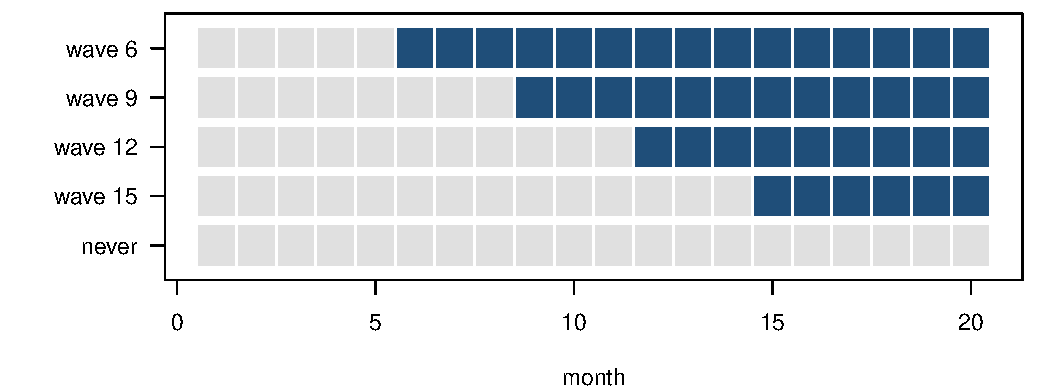
\includegraphics[width=0.66\textwidth]{fig_stag_rollout.pdf}
\end{center}
\end{frame}


\section{What two-way fixed effects estimates}

\begin{frame}{Notation and targets}
\begin{itemize}
	\item $G_i$: the month unit $i$ is first treated (its \alert{cohort}); $G_i = \infty$ if never. Treatment is
	absorbing: $D_{it} = \mathbb{1}\{t \ge G_i\}$. Event time $e = t - G_i$.
	\medskip
	\item The building block is the cohort-by-period effect
	\begin{align*}
		\text{ATT}(g, t) = \E\left[\,Y_{it}(g) - Y_{it}(\infty) \mid G_i = g\,\right], \qquad t \ge g,
	\end{align*}
	where $Y_{it}(\infty)$ is the outcome if never treated.
	\item Summaries you might want, each a \emph{weighted average} of the $\text{ATT}(g,t)$:
	\begin{itemize}
		\item the overall ATT (every treated unit-period counts once);
		\item the effect by cohort;
		\item the effect by event time $e$: the dynamic path.
	\end{itemize}
	\medskip
	\item \alert{Choose the summary before you choose the estimator.} The trouble with two-way FE is that it chooses
	the weights for you.
\end{itemize}
\end{frame}


\begin{frame}{The default regression}
\begin{align*}
	y_{it} = \alpha_i + \gamma_t + \beta \cdot D_{it} + \varepsilon_{it}
\end{align*}
\begin{itemize}
	\item On our rollout: $\hat\beta = 0.024$ (SE 0.003). The truth is 0.061.
	\medskip
	\item Not noise: the standard error is small and every cohort's effect is positive.
	\medskip
	\item Not a failure of parallel trends either. The simulation satisfies parallel trends and no anticipation exactly.
	\medskip
	\item The problem is the \alert{estimand}. To see it, apply Frisch--Waugh--Lovell.
\end{itemize}
\end{frame}


\begin{frame}{FWL: two-way FE is a weighted average with weights you did not choose}
\begin{itemize}
	\item Residualize $D_{it}$ on unit and period effects: $\tilde D_{it} = D_{it} - \bar D_{i\cdot} - \bar D_{\cdot t} + \bar D$
	(balanced panel). Then
	\begin{align*}
		\hat\beta = \frac{\sum_{it} \tilde D_{it}\, y_{it}}{\sum_{it} \tilde D_{it}^2}
		\quad \Rightarrow \quad
		\beta = \sum_{it:\, D_{it} = 1} w_{it}\, \tau_{it}, \qquad w_{it} = \frac{\tilde D_{it}}{\sum_{js:\, D_{js}=1} \tilde D_{js}}.
	\end{align*}
	\item The weights sum to one, but they can be \alert{negative} (de Chaisemartin and D'Haultf{\oe}uille 2020).
	\medskip
	\item Who gets a negative weight? A unit-period where $\bar D_{i\cdot}$ is high (an early adopter) and $\bar D_{\cdot t}$ is high
	(a late month, when most units are treated): $\tilde D_{it} < 0$.
	\medskip
	\item The weights depend only on the \alert{timing}, not on outcomes. You can compute them before you look at $y$.
\end{itemize}
\end{frame}


\begin{frame}{The weights in our rollout}
\begin{columns}[c]
\begin{column}{0.58\textwidth}
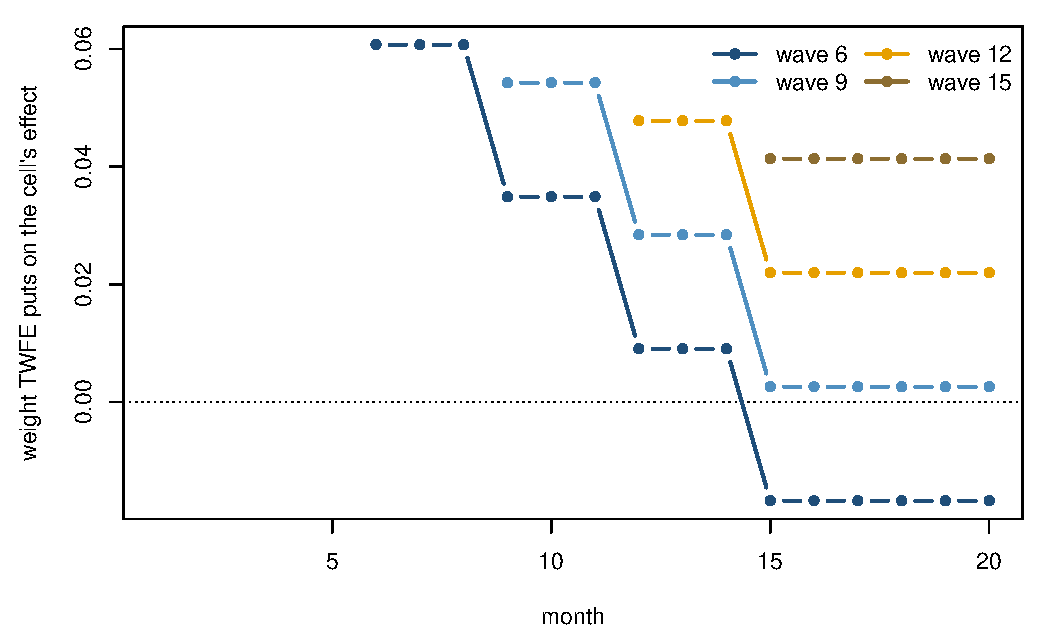
\includegraphics[width=\textwidth]{fig_stag_weights.pdf}
\end{column}
\begin{column}{0.4\textwidth}
\small
\begin{itemize}
	\item Each line is a wave's total weight per month. Wave 6 goes negative once most cities are treated.
	\item 14\% of treated city-months get a negative weight, 8\% of the absolute weight.
	\item Here the negative weights land on the \emph{largest} effects: the early wave, late in its ramp-up. So the
	estimate is pulled down hard.
	\item With a constant effect, any weights summing to one would give the right answer.
\end{itemize}
\end{column}
\end{columns}
\end{frame}


\begin{frame}{Goodman-Bacon (2021): two-way FE as an average of $2\times2$s}
\begin{itemize}
	\item With timing groups $k$ (earlier) and $\ell$ (later) and a never-treated group $U$, the two-way FE estimate is
	\alert{exactly} a weighted average of every $2\times2$ DiD you can form:
	\begin{enumerate}
		\item a timing group vs.\ the never-treated, over the whole panel;
		\item earlier vs.\ later, before the later group is treated: the later group is a \emph{not-yet-treated} control;
		\item later vs.\ earlier, after the earlier group is treated: the earlier group is an \emph{already-treated} control.
	\end{enumerate}
	\medskip
	\item Weights are larger for bigger groups and for pairs whose treatment share is near one half (timing in
	the middle of the panel).
	\medskip
	\item Comparison 3 is the ``forbidden'' one. Its control group's outcomes include its own treatment effects.
\end{itemize}
\end{frame}


\begin{frame}{Why the already-treated comparison is not a treatment effect}
\small
\begin{itemize}
	\item Later group $\ell$ vs.\ earlier group $k$, comparing the window after $\ell$ starts (POST) with the window in between (MID):
	\begin{align*}
		\hat\tau^{\ell}_{k\ell}
		= \big(\bar y_\ell^{\,POST} - \bar y_\ell^{\,MID}\big) - \big(\bar y_k^{\,POST} - \bar y_k^{\,MID}\big).
	\end{align*}
	\item Under parallel trends, the untreated trends cancel and what is left is
	\begin{align*}
		\underbrace{\bar\tau_\ell^{\,POST}}_{\text{a real effect}}
		\;-\; \underbrace{\big(\bar\tau_k^{\,POST} - \bar\tau_k^{\,MID}\big)}_{\text{growth in the control group's effect}}.
	\end{align*}
	\item If effects are constant over time, the second term is zero and the comparison is fine.
	\item If the earlier group's effect is still \emph{growing}, the second term is positive and the comparison is biased
	down. It can even be negative when every true effect is positive.
\end{itemize}
\end{frame}


\begin{frame}{The decomposition in our rollout}
\begin{columns}[c]
\begin{column}{0.56\textwidth}
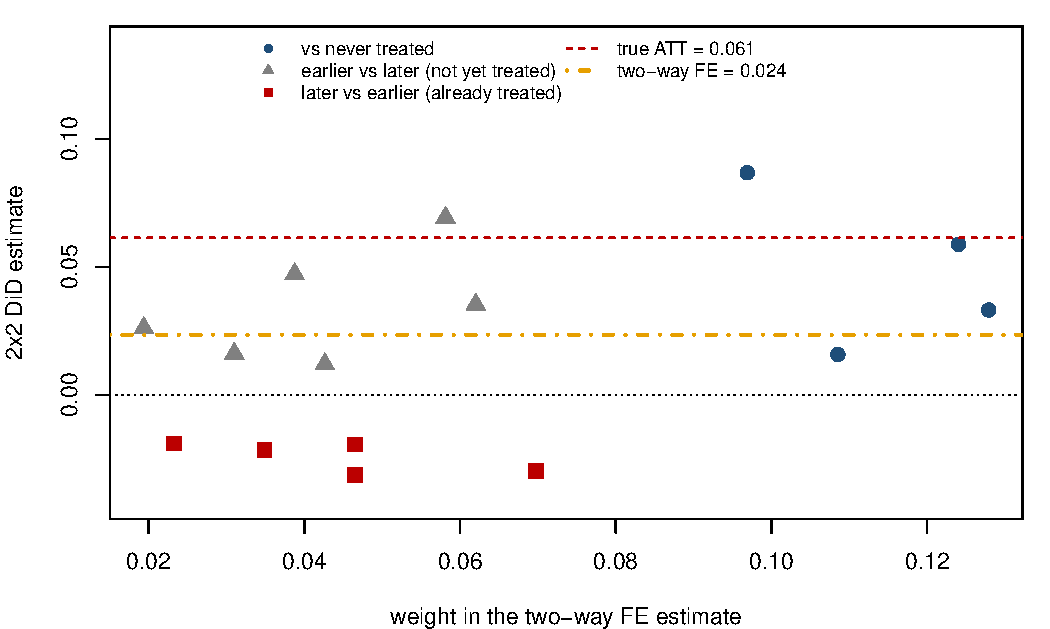
\includegraphics[width=\textwidth]{fig_stag_bacon.pdf}
\end{column}
\begin{column}{0.43\textwidth}
\scriptsize
\begin{tabular}{lccc}\toprule
Control group & $N$ & Weight & Avg. \\ \midrule
vs.\ never treated & 4 & 0.46 & 0.047 \\
vs.\ not yet treated & 6 & 0.25 & 0.038 \\
vs.\ already treated & 6 & 0.29 & -0.026 \\
\bottomrule\end{tabular}

\small
\medskip
\begin{itemize}
	\item All 16 comparisons, weighted, reproduce $\hat\beta = 0.024$ to machine precision.
	\item The already-treated comparisons carry 29\% of the weight and average $-0.026$.
	\item Even the clean comparisons are weighted oddly: the vs.-never 2$\times$2s average 0.047, not 0.061.
\end{itemize}
\end{column}
\end{columns}
\end{frame}


\begin{frame}{Does a dynamic event study fix it?}
\begin{center}
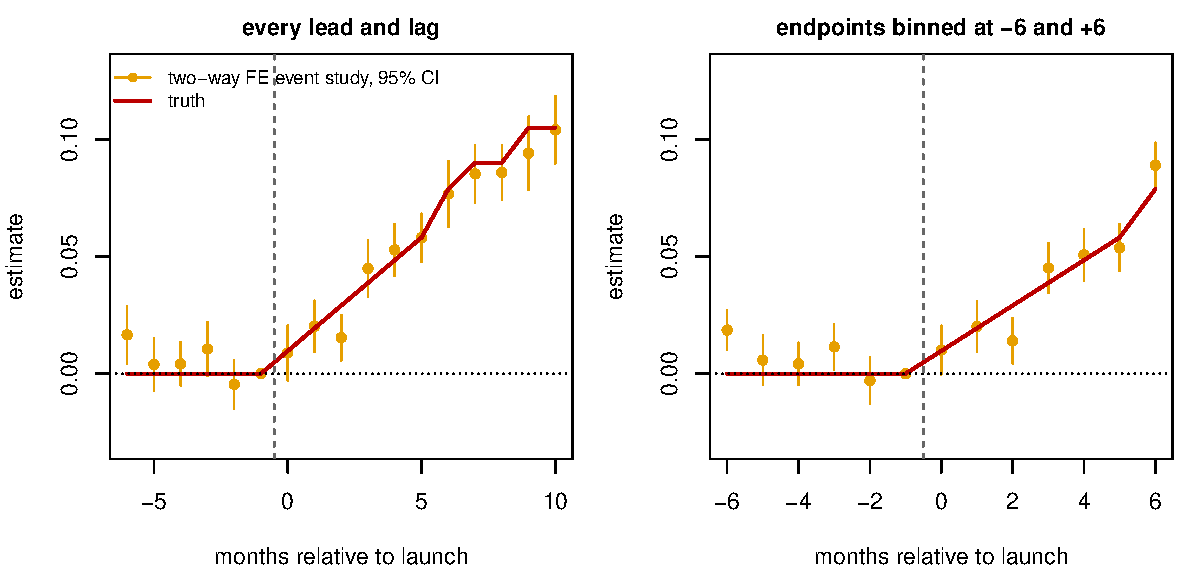
\includegraphics[width=0.8\textwidth]{fig_stag_es_twfe.pdf}
\end{center}
\vspace{-0.3cm}
\footnotesize
\begin{itemize}
	\item Mostly, but not cleanly. With cohorts whose paths differ, each lead or lag coefficient also picks up other cohorts'
	effects at \emph{other} event times (Sun and Abraham 2021). Binning the endpoints, a common shortcut, makes it worse.
	\item A joint test of the leads rejects ($p = 0.04$ left, $p < 0.001$ right), though there is no pre-trend.
\end{itemize}
\end{frame}


\section{The fix: clean comparisons, chosen weights}

\begin{frame}{The fix in one sentence}
\begin{center}
\large
Estimate $2\times2$s that never use already-treated units as controls,\\
then average them with weights \emph{you} choose.
\end{center}
\bigskip
Three ways to do it, which agree in our simulation:
\begin{enumerate}
	\item \alert{Callaway and Sant'Anna (2021)}: estimate each $\text{ATT}(g,t)$ as its own $2\times2$, then aggregate.
	\item \alert{Sun and Abraham (2021)}: the same thing, written as one fully interacted regression.
	\item \alert{Imputation} (Borusyak, Jaravel and Spiess 2024; Gardner, Thakral, T\^o and Yap 2024;
	Wooldridge 2025): fit the untreated outcome model on untreated observations only, predict $Y(0)$ for the treated,
	and average the gaps.
\end{enumerate}
\end{frame}


\begin{frame}{Callaway and Sant'Anna: ATT$(g,t)$ one $2\times2$ at a time}
\begin{itemize}
	\item For cohort $g$ and period $t$, compare the change since the last pre-period $g-1$ with the change in a
	clean comparison group $\mathcal{C}$:
	\begin{align*}
		\widehat{\text{ATT}}(g,t) = \Big(\bar y_{g,t} - \bar y_{g,g-1}\Big) - \Big(\bar y_{\mathcal{C},t} - \bar y_{\mathcal{C},g-1}\Big).
	\end{align*}
	\item Two choices of $\mathcal{C}$:
	\begin{itemize}
		\item \alert{never-treated} units ($G = \infty$);
		\item \alert{not-yet-treated} units ($G > t$). More controls, more power, but parallel trends must hold for more groups,
		and none of them may anticipate treatment.
	\end{itemize}
	\medskip
	\item Assumptions: parallel trends between each cohort and its comparison group, and no anticipation.
	Covariates enter through outcome regression, weighting, or both (doubly robust, as in 9a).
\end{itemize}
\end{frame}


\begin{frame}{ATT$(g,t)$ in our rollout}
\begin{center}
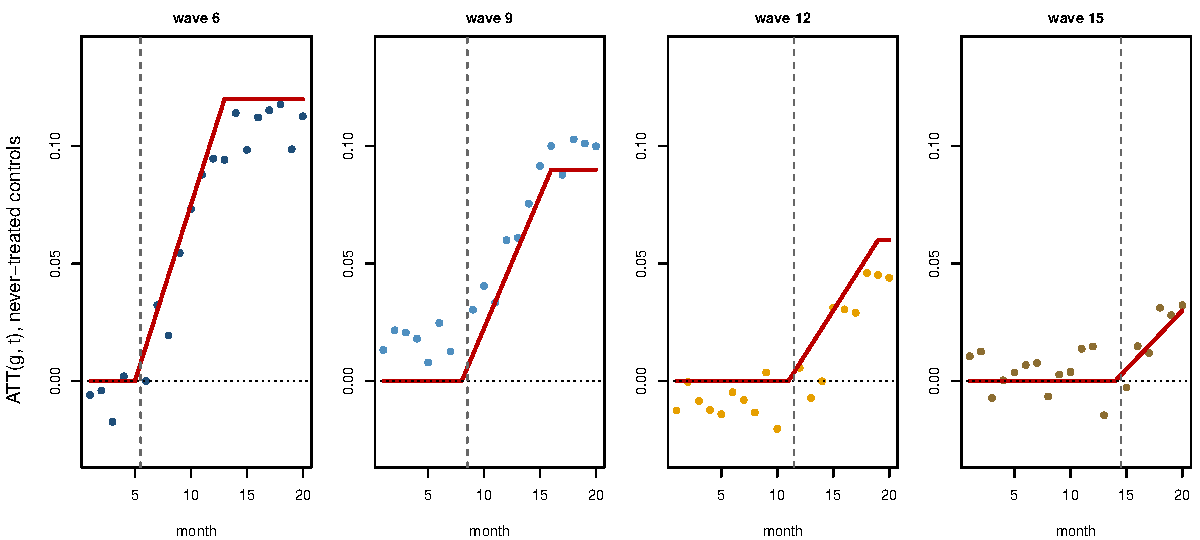
\includegraphics[width=0.95\textwidth]{fig_stag_attgt.pdf}
\end{center}
\vspace{-0.2cm}
{\small One panel per wave; red is the truth. Each point is a $2\times2$ against the never-treated cities. Pre-period points are
placebo $2\times2$s relative to month $g-1$.}
\end{frame}


\begin{frame}{Aggregating ATT$(g,t)$}
\small
With cohort shares $P(G = g)$ as weights and $\mathcal{T}$ periods:
\begin{itemize}
	\item \alert{Overall}: average every post-period $\text{ATT}(g,t)$, weighting by cohort size. Each treated unit-period counts once.
	\item \alert{By cohort}: $\theta(g) = \frac{1}{\mathcal{T} - g + 1} \sum_{t \ge g} \text{ATT}(g,t)$.
	\item \alert{By event time}: the dynamic path
	\begin{align*}
		\theta(e) = \sum_{g} \mathbb{1}\{g + e \le \mathcal{T}\}\, P(G = g \mid G + e \le \mathcal{T})\, \text{ATT}(g, g+e).
	\end{align*}
	\item \alert{By calendar period}: $\theta(t)$, averaging over cohorts treated by $t$.
\end{itemize}
\medskip
Caveats:
\begin{itemize}
	\item The cohorts behind $\theta(e)$ change with $e$. In our data only wave 6 is observed at $e = 14$.
	\item Long-horizon points describe early adopters, who may differ. Balance the panel in event time if you want a fixed composition.
\end{itemize}
\end{frame}


\begin{frame}{Sun and Abraham: the same thing as a regression}
\begin{itemize}
	\item Interact cohort with event time, and use only clean controls:
	\begin{align*}
		y_{it} = \alpha_i + \gamma_t + \sum_{g} \sum_{e \neq -1} \delta_{g,e} \cdot \mathbb{1}\{G_i = g\} \cdot \mathbb{1}\{t - G_i = e\} + \varepsilon_{it},
	\end{align*}
	with never-treated (or last-treated) units as the comparison. Then average $\hat\delta_{g,e}$ across cohorts with
	cohort-share weights.
	\medskip
	\item Every treated cell except $e = -1$ has its own dummy, so the $\gamma_t$ are estimated from clean controls only.
	\medskip
	\item With never-treated controls and no covariates, $\hat\delta_{g,e}$ is \emph{numerically} the Callaway--Sant'Anna
	$\widehat{\text{ATT}}(g, g+e)$ with base period $g-1$. In our simulation they agree to 12 decimal places.
	\medskip
	\item In \texttt{fixest}: \texttt{feols(y $\sim$ sunab(cohort, month) | city + month)}. Assignment 5 uses it.
\end{itemize}
\end{frame}


\begin{frame}{Imputation}
\begin{enumerate}
	\item Fit $y_{it} = \alpha_i + \gamma_t + \varepsilon_{it}$ on the \alert{untreated} observations only (never-treated, plus
	treated units before their date).
	\item Predict $\hat Y_{it}(0) = \hat\alpha_i + \hat\gamma_t$ for every treated observation.
	\item $\hat\tau_{it} = y_{it} - \hat Y_{it}(0)$. Average with whatever weights you want: overall, by cohort, by event time.
\end{enumerate}
\medskip
\begin{itemize}
	\item Borusyak, Jaravel and Spiess (2024) give the efficiency theory. Gardner et al.'s two-stage DiD (\texttt{did2s}) is the
	same idea, and so is Wooldridge's (2025) extended two-way FE regression, a Mundlak-style version.
	\medskip
	\item Assumption: parallel trends in \emph{all} periods, not just relative to $g-1$. In exchange it uses every pre-period as a
	baseline, which buys precision when errors are not strongly serially correlated.
	\medskip
	\item Needs untreated observations for every unit and period it predicts: always-treated units drop out.
\end{itemize}
\end{frame}


\begin{frame}{The horse race: event-time paths}
\begin{center}
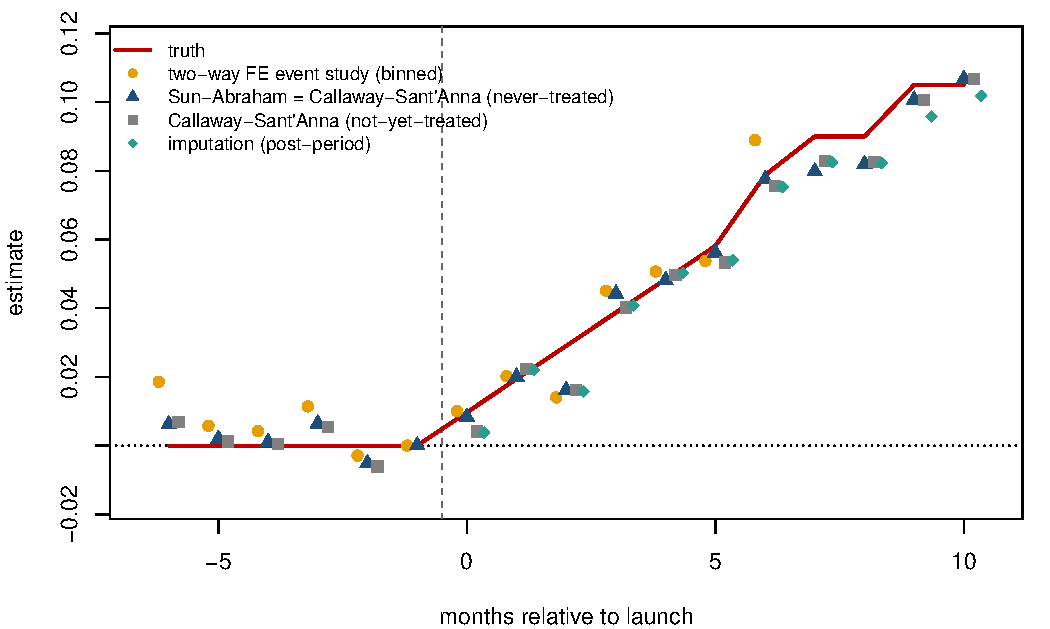
\includegraphics[height=0.78\textheight]{fig_stag_horse.pdf}
\end{center}
\vspace{-0.3cm}
{\small Every clean estimator tracks the truth (red); the binned two-way FE event study drifts in the pre-period.}
\end{frame}


\begin{frame}{The horse race: one number}
\begin{center}
\footnotesize
\begin{tabular}{lccc}\toprule
Estimator & Overall ATT & Std.\ error & Bias \\ \midrule
Static two-way FE & 0.024 & (0.003) & -0.038 \\
Sun--Abraham (\texttt{sunab}), never-treated controls & 0.058 & (0.005) & -0.003 \\
Callaway--Sant'Anna, never-treated controls & 0.058 & (0.005) & -0.003 \\
Callaway--Sant'Anna, not-yet-treated controls & 0.058 & (0.005) & -0.004 \\
Imputation (Borusyak--Jaravel--Spiess) & 0.057 & (0.004) & -0.004 \\
\midrule
Truth: mean effect over treated city-months & 0.061 & &  \\
\bottomrule\end{tabular}
\\[2pt]
{\scriptsize SEs for the hand-coded estimators: cluster bootstrap over cities (199 draws).}
\end{center}
\small
\begin{itemize}
	\item Static two-way FE gives \emph{less than half} the truth, with a small standard error.
	\item The clean estimators agree with each other. If they disagreed, an assumption would be doing work; find out which.
	\item Imputation is the most precise (SE 0.004 vs.\ 0.005), the payoff from its stronger assumption: it uses every
	pre-period, not just $g-1$.
\end{itemize}
\end{frame}


\section{Practice}

\begin{frame}{Choosing the comparison group}
\begin{itemize}
	\item \alert{Never-treated.} Cleanest, but ask why they never adopted. Never-adopters are often different (smaller,
	rural, uninterested), and parallel trends with them is a strong claim.
	\medskip
	\item \alert{Not-yet-treated.} Units that will adopt soon are often more comparable. Requires no anticipation.
	\medskip
	\item \alert{No never-treated group}: use the last cohort as the control until it is treated. Effects after that date are not
	identified without extrapolation.
	\medskip
	\item \alert{Always-treated units} (adopted before the sample starts) cannot be a clean control and have no pre-period. Drop
	them. Two-way FE instead uses them as controls throughout.
	\begin{itemize}
		\item In a variant of our rollout with 50 always-treated cities, 24\% of treated rows get negative weights and two-way FE
		gives 0.015 (truth 0.061). Imputation without them gives 0.060.
	\end{itemize}
	\medskip
	\item \alert{Anticipation}: if units react $\delta$ periods early, use $g - 1 - \delta$ as the base period.
\end{itemize}
\end{frame}


\begin{frame}{Pre-period plots are not comparable across estimators}
\begin{itemize}
	\item Regression event studies (two-way FE, Sun--Abraham) report every coefficient relative to $e = -1$: long differences
	on both sides.
	\medskip
	\item \texttt{did::att\_gt} by default uses a \alert{varying} base period: pre-period points are \emph{short} differences
	($t$ vs.\ $t-1$), post-period points are long differences ($t$ vs.\ $g-1$). A steady pre-trend then looks flat before and
	kinked after.
	\medskip
	\item Imputation's pre-trend test is a different object again: it regresses untreated outcomes on leads.
	\medskip
	\item So do not eyeball a ``flat pre-period'' across methods. For plots comparable to a regression event study, set
	\texttt{base\_period = "universal"} (Roth 2026 WP, ``Interpreting Event-Studies from Recent Difference-in-Differences Methods'').
	Our figures use the universal base.
\end{itemize}
\end{frame}


\begin{frame}{Before you estimate anything}
\begin{enumerate}
	\item \alert{Plot the rollout.} Which cohorts, how big, and when? (\texttt{panelview}.)
	\item \alert{Count} never-treated and always-treated units. Few never-treated units and many always-treated ones are where
	two-way FE goes wrong.
	\item \alert{Compute the two-way FE weights.} They depend only on timing. Report the share that is negative.
	\item \alert{Run the Goodman-Bacon decomposition.} How much weight sits on already-treated comparisons, and do those
	$2\times2$s disagree with the clean ones?
	\item Estimate with a clean estimator. Report the event-time path \emph{and} your chosen aggregate. Put two-way FE beside it.
	\item If they differ, the decomposition tells you why. If they agree, say so: it is reassuring.
\end{enumerate}
\end{frame}


\begin{frame}{Does the TWFE Problem Matter in Practice? (Hull 2026)}
\footnotesize
\begin{itemize}
\item AI-assisted replication of 1,346 staggered-adoption specs from 108 papers (about half of the specs from top-five journals).
\item Compare TWFE to DiD-averaging (Callaway--Sant'Anna) and imputation (Borusyak--Jaravel--Spiess).
\end{itemize}
\smallskip
\begin{center}
\begin{tabular}{lcc}
\toprule
 & DiD-averaging & Imputation \\
\midrule
Correlation with TWFE estimate & 0.88 & 0.93 \\
Sign flips & 14.5\% & 10.8\% \\
Sign flips with a significant difference & 3.5\% & 2.2\% \\
Modern SE relative to TWFE SE & +47\% & +14\% \\
\bottomrule
\end{tabular}
\end{center}
\smallskip
\begin{itemize}
\item Negative weights are small in the median static spec: 8\% of treated rows, 1.4\% of absolute weight.
\item The tradeoff: robustness to TWFE's implicit weighting vs.\ the precision of OLS.
\end{itemize}
\end{frame}


\begin{frame}{Separating Noise from True Differences (Hull 2026)}
\footnotesize
\begin{itemize}
\item Hierarchical model: $\hat\theta_k \mid \theta_k \sim N(\theta_k, S_k)$ for each (TWFE, modern) pair; bivariate normal prior on $\theta_k$.
\end{itemize}
\smallskip
\begin{center}
\begin{tabular}{lcc}
\toprule
Estimands & DiD-averaging & Imputation \\
\midrule
Correlation of TWFE and modern estimands & 0.91 & 0.98 \\
Sign reversal & 11.5\% & 5.6\% \\
Significant TWFE estimate with the wrong sign & 2.1\% & 0.6\% \\
\bottomrule
\end{tabular}
\end{center}
\smallskip
\begin{itemize}
\item \alert{When to worry:} +10pp always-treated share $\Rightarrow$ +6.7pp sign flips (DiD-averaging; forbidden comparisons); +10pp never-treated share $\Rightarrow$ $-2.1$pp (imputation).
\item Flips are rarer after 2021 and when papers report both estimators. Caveat: these are \emph{published} specifications.
\item Run the modern estimator anyway (it's cheap), but old TWFE results are not presumptively wrong.
\end{itemize}
\end{frame}


\begin{frame}{Our simulation vs.\ Hull's sample}
\begin{itemize}
	\item Our rollout was built to break two-way FE:
	\begin{itemize}
		\item effects that grow for eight months;
		\item larger effects for earlier waves;
		\item a short panel in which most cities end up treated.
	\end{itemize}
	There, 14\% of treated rows carry negative weight; in Hull's median spec, 8\%.
	\medskip
	\item The lesson is not ``two-way FE is always badly wrong.'' It is: two-way FE is right under \emph{constant} effects,
	and you can check cheaply how far from that you are.
	\medskip
	\item The diagnostics on the previous slides tell you which world you are in before a referee does.
\end{itemize}
\end{frame}


\begin{frame}{Beyond binary, absorbing treatments (pointers)}
\begin{itemize}
	\item \alert{Treatments that switch on and off}, or units whose treatment changes more than once: de Chaisemartin and
	D'Haultf{\oe}uille (2020, \emph{AER}; 2026, \emph{REStat}), which compare switchers with units whose treatment has not yet changed.
	\medskip
	\item \alert{Continuous treatment} (dose: ad spend, a tax rate): Callaway, Goodman-Bacon and Sant'Anna (2024 WP). Comparing
	dose levels needs a stronger parallel-trends assumption than comparing treated with untreated.
	\medskip
	\item \alert{Sensitivity to violations of parallel trends}: \texttt{HonestDiD} (Rambachan and Roth 2023; Session 8).
	\medskip
	\item \alert{Few treated units, long pre-period}: synthetic control and synthetic DiD (Session 11).
	\medskip
	\item Survey: Roth, Sant'Anna, Bilinski and Poe (2023, \emph{JoE}), ``What's trending in difference-in-differences?''
\end{itemize}
\end{frame}


\begin{frame}[fragile]{In practice}
\begin{lstlisting}
# cohort g = first treated month; never-treated: g = 0 for did/didimputation, g = 10000 for sunab
fit <- feols(y ~ sunab(g_sa, month) | city + month, d, vcov = ~city)             # Sun-Abraham
summary(fit, agg = "ATT")                                                          # overall ATT
att <- did::att_gt(yname = "y", tname = "month", idname = "city", gname = "g", data = d,
                   control_group = "notyettreated", base_period = "universal")
did::aggte(att, type = "dynamic")                                                 # also "simple", "group", "calendar"
didimputation::did_imputation(data = d, yname = "y", gname = "g", tname = "month", idname = "city",
                              horizon = TRUE, pretrends = -5:-1)                  # imputation
bacondecomp::bacon(y ~ D, data = d, id_var = "city", time_var = "month")           # Goodman-Bacon weights
\end{lstlisting}
\begin{lstlisting}[language=Python]
pf.panelview(d, unit="city", time="month", treat="D")                             # the rollout
fit = pf.event_study(d, yname="y", idname="city", tname="month", gname="g", estimator="did2s")
fit = pf.did2s(d, yname="y", first_stage="~ 0 | city + month",
               second_stage="~ i(rel, ref=-1.0)", treatment="D", cluster="city")
\end{lstlisting}
\end{frame}


\begin{frame}{Recap}
\begin{itemize}
	\item With staggered timing and effects that change, static two-way FE is a weighted average of cohort-period effects
	with timing-driven weights. Some are negative, and the already-treated comparisons are not treatment effects.
	\medskip
	\item Dynamic two-way FE event studies are better but still mix cohorts, and binning makes it worse.
	\medskip
	\item Fix: clean $2\times2$s (never- or not-yet-treated controls), aggregated with weights you choose. Callaway--Sant'Anna,
	Sun--Abraham and imputation all do this; imputation trades a stronger assumption for precision.
	\medskip
	\item Before estimating: plot the rollout, count never- and always-treated units, compute the weights, decompose.
	\medskip
	\item In published work the damage is usually modest (Hull 2026). Run the modern estimator and report both.
\end{itemize}
\end{frame}


\begin{frame}{Workbook time}
\texttt{Fall/L9 - Quasi Experiments/inclass\_session9.Rmd}, Part 2 (Python: \texttt{inclass\_session9\_py.qmd}):
\begin{enumerate}
	\item Reproduce static two-way FE, \texttt{sunab}, hand-coded Callaway--Sant'Anna and imputation on the rollout, against the truth.
	\item Make the effect constant across waves and over time. Which estimators change, and why?
	\item Drop the never-treated cities. Which comparisons are left, and which event-time effects can you still estimate?
\end{enumerate}
\end{frame}

\end{document}
